%!TEX root = ../main.tex

\subsection{Vacromium}
\label{ssec:vacromium}

Next, a vacromium absorber is placed in the beam path\footnote{The vacromium
Mössbauer spectrum was measured last (and longest) during the lab exercise. In order
to streamline the text it is however decided to discuss the material in this section
already.}. The analysis of data proceeds as presented in \autoref{ssec:iron}. One
absorption peak can be discovered in the vacromium Mössbauer spectrum as seen in
\autoref{fig:vacromium} and \autoref{tab:vacromium}.

The isometric shift for Vacromium can be determined in the same way it was determined
for iron in \autoref{ssec:iron}. The isometric shift of the absorption peaks is hence

\begin{equation}
\Delta E = \SI{10.38\pm1.652e-09}{\electronvolt}
\end{equation}

\todo{Discussion of isometric shift?}

The FWHM for Ch1 and Ch2 in terms of photon energy caused by the Doppler shift is

\begin{align*}
\Gamma_\text{Ch1} &= \SI{5.250\pm1.009e-9}{\electronvolt} \\
\Gamma_\text{Ch2} &= \SI{5.041\pm1.644e-9}{\electronvolt}.
\end{align*}

It follows a mean value of $\Gamma = \SI{5.146\pm0.965e-9}{\electronvolt}$. From
this the mean lifetime $\tau$ of the metastable \SI{14.4}{\kilo\electronvolt}
$^{57}$Fe-state is given by the time-energy uncertainty relation.

\begin{equation}
\label{eq:tau-iron}
\tau\cdot\Gamma = \hbar \Leftrightarrow \tau = \frac{\hbar}{\Gamma} = \SI{127.91\pm23.98}{\nano\second}
\end{equation}

This lies within the expectation of a literature value $\tau=\SI{141}{\nano\second}$
extracted from \cite{nishida1981moessbauer}.

\begin{figure}
	\centering
	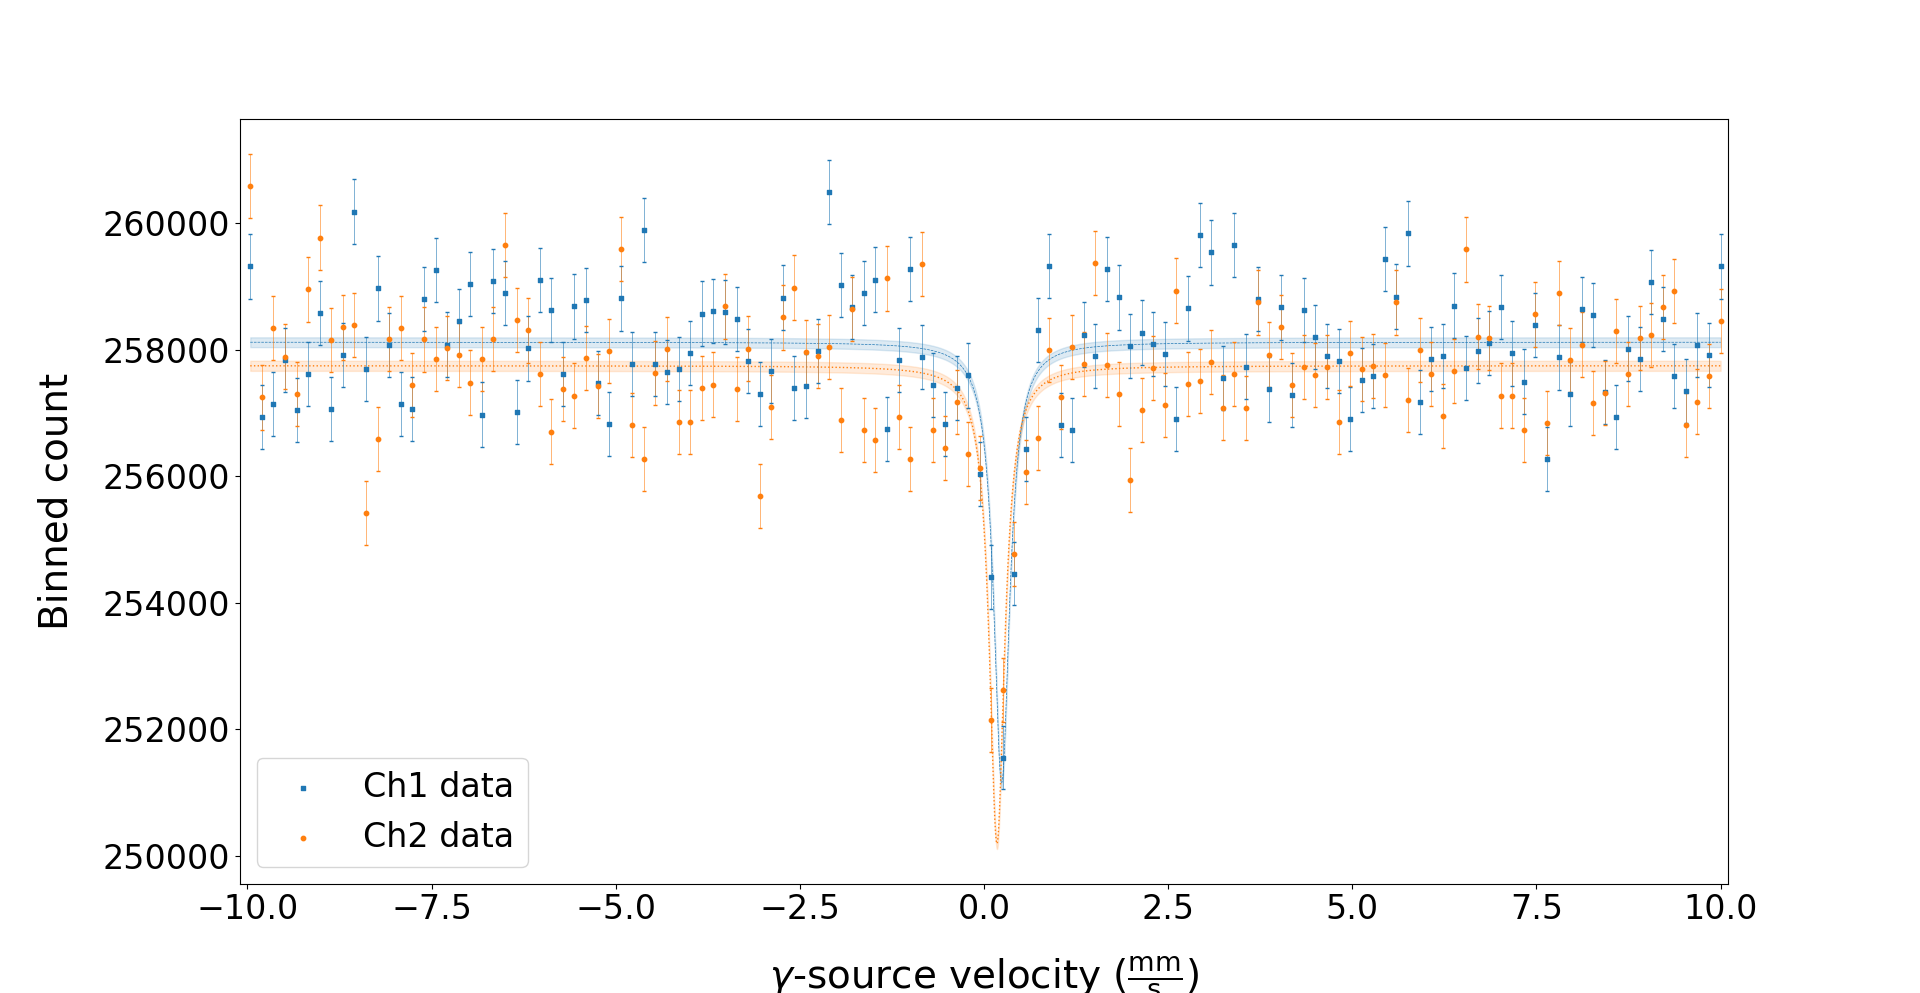
\includegraphics[width=1.0\textwidth]{./fig/Vacromium.png}
	\caption{Mössbauer spectrum of vacromium}
	\label{fig:vacromium}
\end{figure}

\begingroup
\renewcommand{\arraystretch}{1.3}
\begin{table}
	\begin{center}
	\caption{Mössbauer spectrum fit parameters for vacromium}
	\begin{tabular*}{0.9\textwidth}{@{\extracolsep{\fill}} c|ccccc}
  \toprule
	\hline
  Peak \# & $\Upphi_0$ & $A$ & $v_0$ & $\Gamma$ & Channel \\
	\hline
  \multirow{2}{*}{\#1} & $258122\pm78$ & $120\pm39.1$ & $0.24\pm0.03$ & $0.262\pm0.050$ & Ch1 \\
                       & $257749\pm80$ & $120\pm54.1$ & $0.18\pm0.01$ & $0.252\pm0.082$ & Ch2 \\
                       \hline
    \bottomrule
		\end{tabular*}
		\label{tab:vacromium}
	\end{center}

\end{table}
\endgroup

